% Chapter 5

\chapter{Results} % Main chapter title

\label{results} % For referencing the chapter elsewhere, use \ref{Chapter1} 

\lhead{Chapter 6. \emph{Results and Discussion}} % This is for the header on each page - perhaps a shortened title

%----------------------------------------------------------------------------------------


\section{Mesh projection routine}
As an initial test of the algorithm a mesh was created based on the hill of Ekeberg.
The surface was loaded as a \verb|.tin| file in ICEM and a simple box was created with 
the described terrain as floor. The domain with the initial mesh in given in 
figure~\ref{fig:surfpro}. This geometry was chosen because it resembles a typical problem with 
spectral elements. Since the initial element-mesh is relatively coarse it does not capture all 
the details in the geometry and the GLL-nodes distributed on the faces corresponding to the 
unstructured surface will be misplaced. 
%It is however no theoretical problem to reconstruct the surface with with a polynomial of order $P$. 
With the routine described in \cref{surfpro} the surface was approximated accurately by higher order polynomials.
%
\begin{figure}
\centering
  \centerline{
\begin{minipage}{.5\textwidth}
  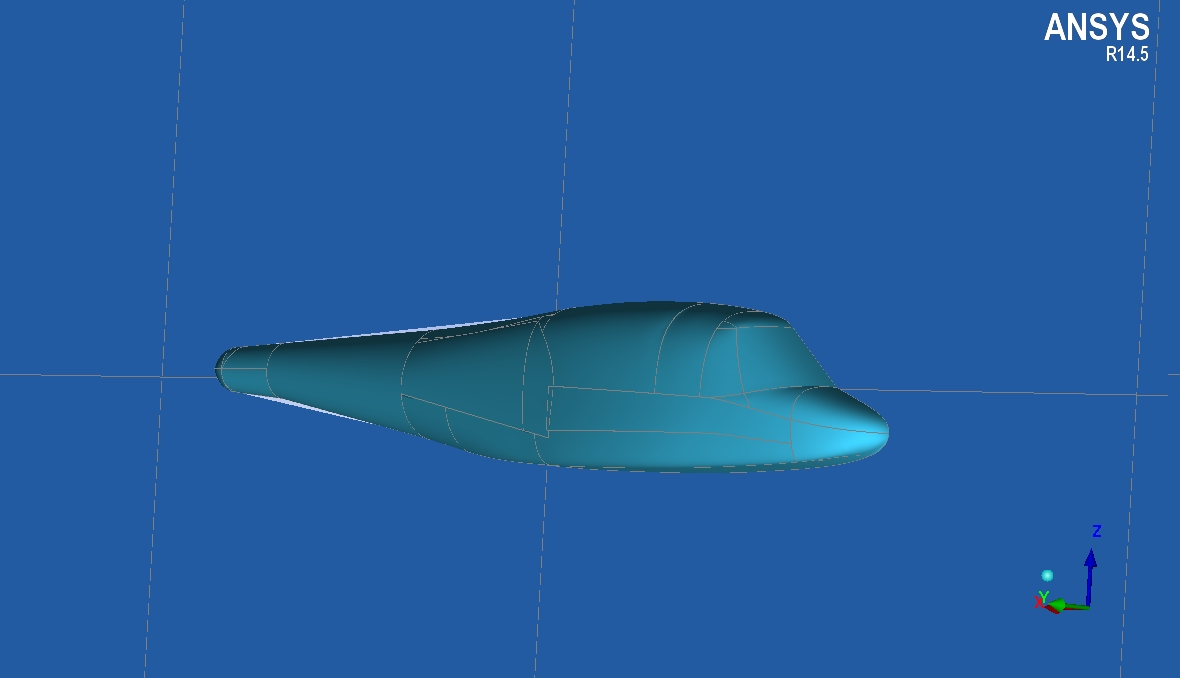
\includegraphics[width=0.9\linewidth]{Figures/helicopter.jpg}
  %\captionof{figure}{A figure}
\end{minipage}%
\begin{minipage}{.5\textwidth}
  \centering
  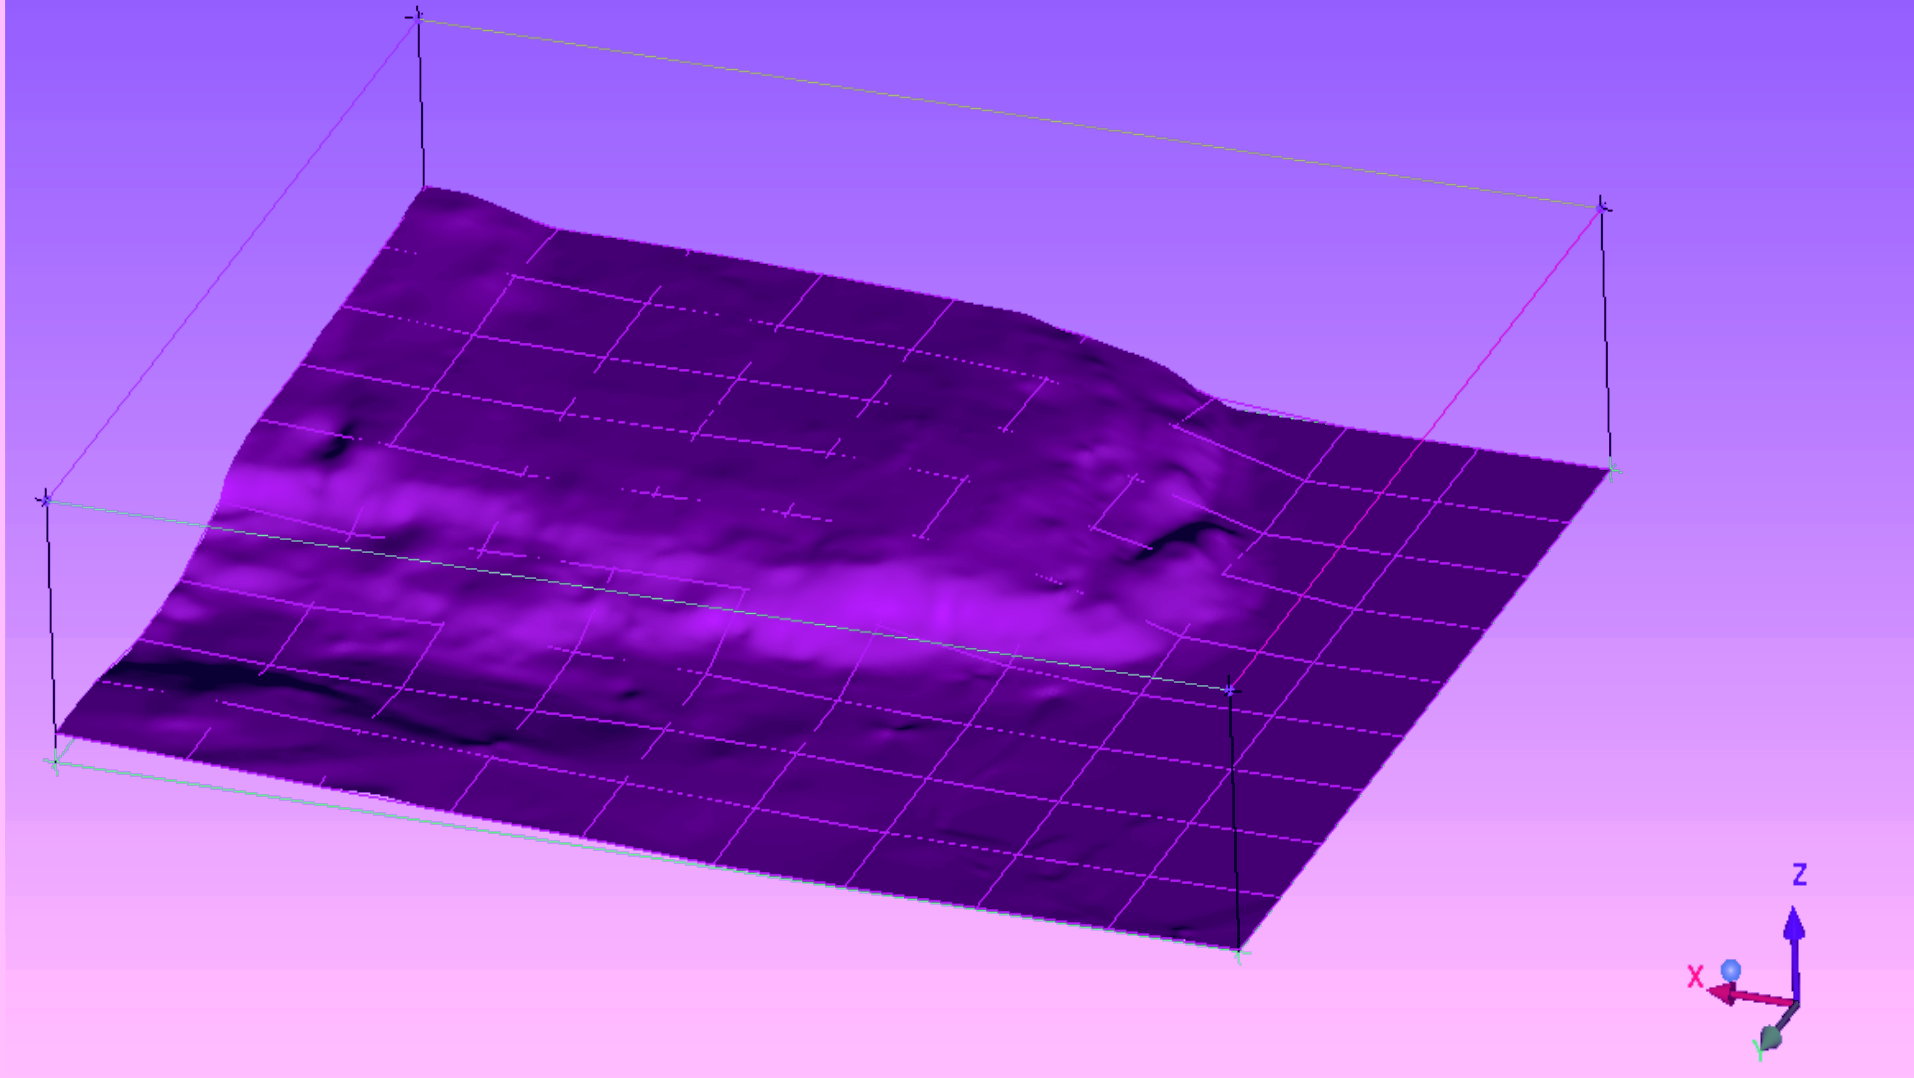
\includegraphics[width=0.9\linewidth]{Figures/mesh_ekebergaasen2.png}
\end{minipage}
}
  \caption{Two examples of smooth surfaces with no analytical expression. 
  To the left is the body of a helicopter, to the right is the hill of Ekeberg.}
  \label{fig:surfpro}
\end{figure}
%
The algorithm restricts itself to relatively smooth surfaces.
\section{Drag and lift on a cylinder}
The effect of the algorithm explained in Chapter~\ref{xyzarc} is
illustrated by solving a laminar flow test problem. 
The solution is compared with previously benchmark computations performed by a number of 
contributors~\cite{benchmark}. 

The results are presented in table~\ref{tab:testcase}, and they confirm that the treatment of the geometry is 
essential, both coefficients are computed with significantly better accuracy. 
%
\begin{table}
\centering
\begin{tabular}{l l c c c c}
		\toprule
		\# of Cells & Software & $c_D$ & $c_L$ & \%\textbf{Err} $c_D$ &\%\textbf{Err} $c_L$ \\ \midrule 
		2070 & Nek5000 (mid) & 6.18349 & 0.008939 & 0.030 & 4.19 \\ 
		2070 & Nek5000 (arc) & 6.18498 & 0.009413 & 0.006 & 0.13 \\
		3145728 & CFX 		 & 6.18287 & 0.009387 & 0.04 &0.15 \\
		3145728 & OF	     & 6.18931 & 0.00973 & 0.06 &3.5 \\
		3145728 & FEATFLOW   & 6.18465 & 0.009397 & 0.01 &0.05 \\
		\bottomrule	
	\end{tabular}
	\caption{Results for the drag and lift coefficients with reference values 
	$c_D = 6.18533$ and $c_L = 0.009401$. $p=11$ for the simulations in Nek.}
\label{tab:testcase}
\end{table}
%
Compared with the results from the other softwares applied in~\cite{benchmark} Nek5000 performs 
just as well or better in most cases. It should be mentioned that the division of the grid is created
in a different manner for Nek5000 so the comparison is not as direct as it may seem from the table.

\subsection{Parameter adjustments in Nek5000}
As discussed in \cref{nek} there are many adjustments available in Nek. 
In order to enlighten the actual effect on the results, several different settings was
investigated for this case and the results are presented in table~\ref{tab:perf}. 
The spectral convergence is also confirmed in figure~\ref{fig:liftconv} by calculating the 
lift coefficient error for increasing polynomial degree. 
%
\begin{figure}[h]
	\centerline{
        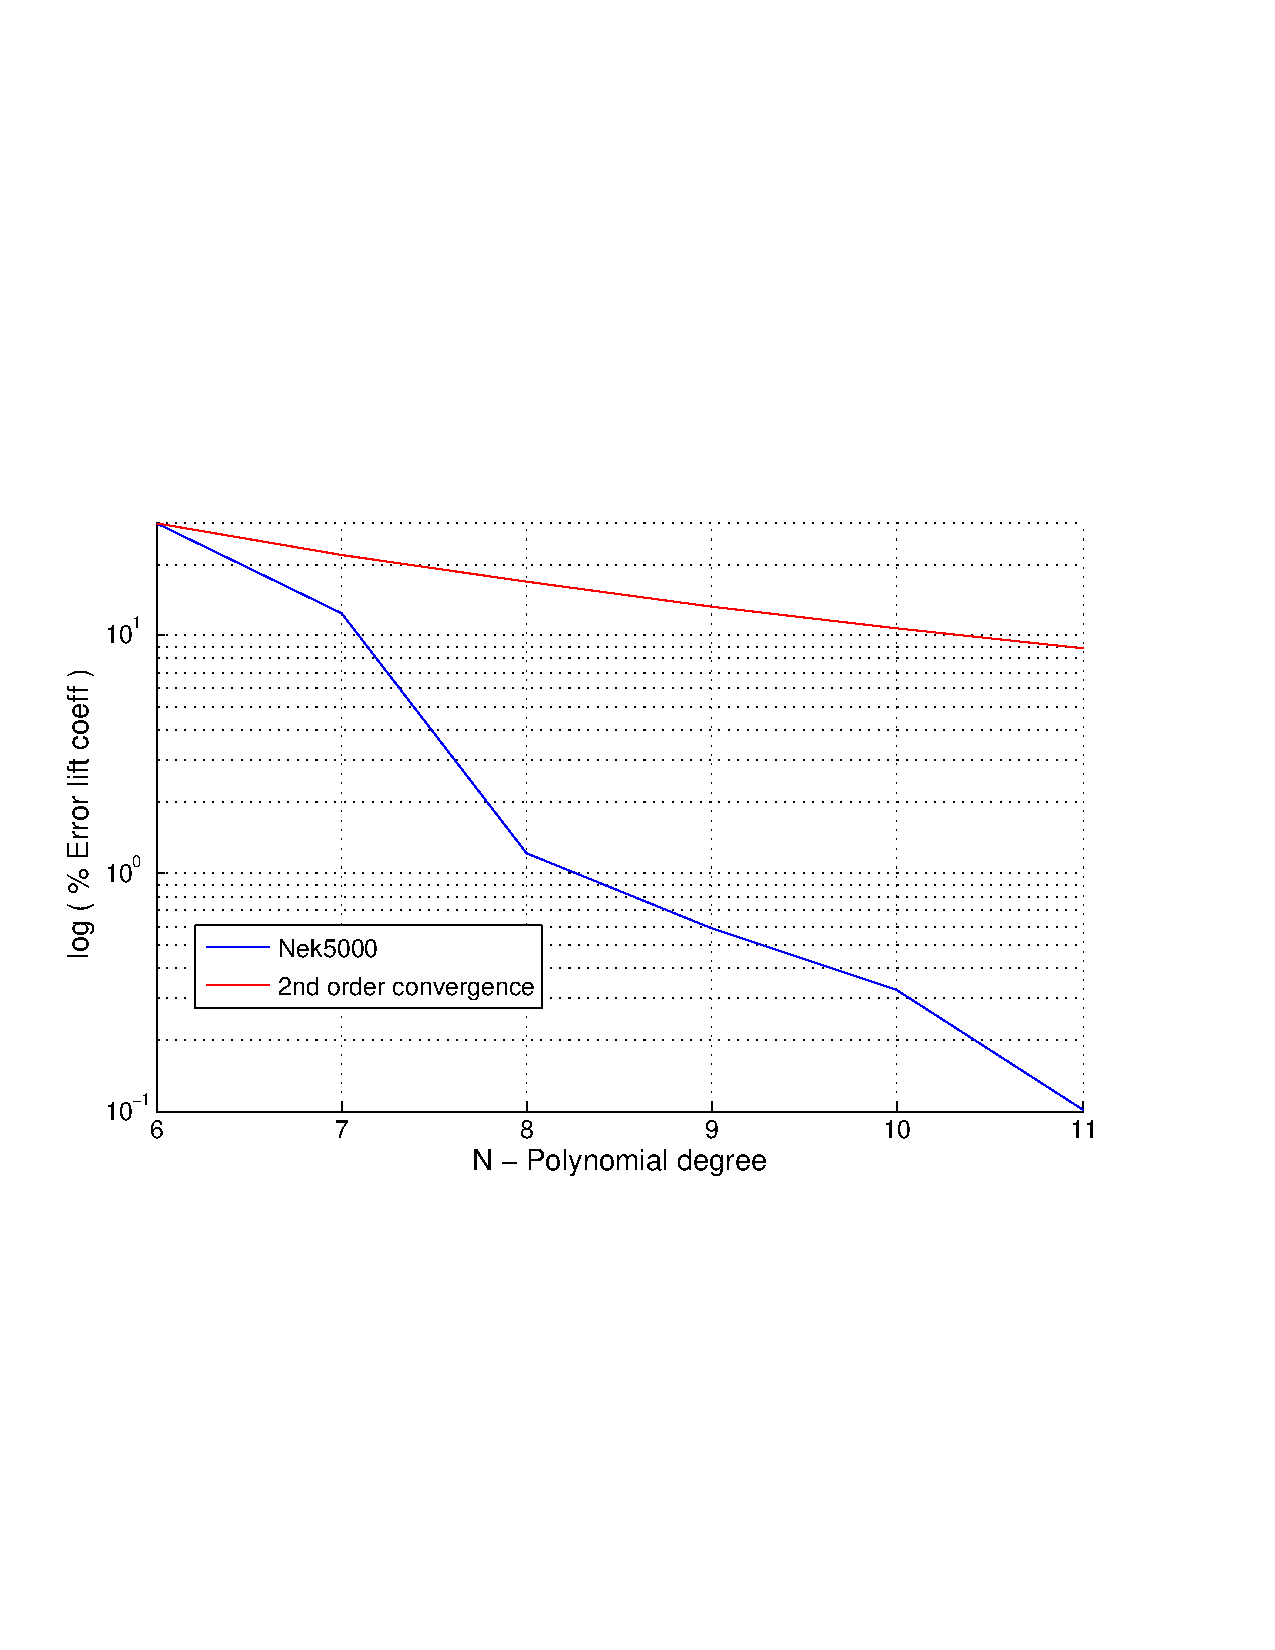
\includegraphics[trim=0.5cm 7cm 0.5cm 7cm, width=0.8\textwidth]{Figures/lift_coef2.pdf}}
	\caption{The logarithm of the error plotted against the polynomial degree. All results 
        are with $P_NP_{N-2}$ and dealiasing, and they are solved without using the 
    characteristic scheme or any filtering. A line illustrating a second order convergence is 
    plotted to verify the convergence rate.}
	\label{fig:liftconv}
\end{figure}
%

The setting that has the biggest impact on the result is the $P_NP_N$ scheme which clearly performs 
worse than the others. This is as expected because of the splitting scheme applied, which 
induces nonvanishing errors in the pressure close to the boundary. 
Use of the IOFS method also has a negative effect on the accuracy,
this is also as expected because of the stability-accuracy tradeoff for this method.
Remember that this scheme allows a much higher time step. The filtering is the least significant change
which confirms the analytical results from \eref{eq:filterenergy}. 
%
\begin{table}[h]
    \centering
    \begin{tabular}{c | c c c c | c c }
         & \multicolumn{4}{|c|}{Settings} & \multicolumn{2}{|c}{\% Error} \\\hline
         \#  & ifsplit & Dealiasing & IOFS & Filter & $c_D$ & $c_L$ \\  \hline 
         1 & No & Yes& No & No & 0.005 & 0.10\\
         2 & Yes& Yes& No & No & 0.013 & 2.35\\
         3 & No & Yes& No & Yes& 0.005 & 0.43\\
         4 & No & Yes& Yes& No & 0.005 & 0.18\\
         !!!5 & No & No & No & No & 0.005 & 0.03\\
         6 & Yes tstep=3e-4& Yes& No & No & 0.004 & 0.487\\
    \end{tabular}
    %\begin{tabular}{c | c c c c | c c | c c c}
         %& \multicolumn{4}{|c|}{Settings} & \multicolumn{2}{|c|}{\% Error} & \multicolumn{3}{|c}{Data} \\\hline
         %\#  & ifsplit & Dealiasing & IOFS & Filter & $c_D$ & $c_L$ & DT & CFL & T/Tstep \\ \hline 
         %1 & F & T & F & F & 0.005 & 0.102 & 1e-04 & 2.03 & 2.1e-02 \\
         %2 & T & T & F & F & 0.013 & 2.349 & 1e-04 & 2.03 & 2.1e-02 \\
         %3 & F & T & F & T & 0.005 & 0.431 & 1e-04 & 2.03 & 2.1e-02 \\
         %4 & F & T & T & F & 0.005 & 0.179 & 1e-04 & 2.03 & 2.1e-02 \\
         %5 & F & F & F & F & NaN   & NaN   & 1e-04 & 2.03 & 2.1e-02 \\
    %\end{tabular}
    \caption{Test of solver settings in Nek5000.}
    \label{tab:perf}
\end{table}
%

Be aware that these results are obtained from a laminar test case and does not in any way 
suggest any optimal adjustment for Nek5000. The results are included to gain a better understanding
of how the different settings can affect the solution.

%----------------------------------------------------------------------------------------
\section{Gas dispersion in a simplified urban area} 
This case is a part of a larger project designed to evaluate different solvers 
ability to perform simulations of gas dispersion. The N-S equations are solved using
the $P_NP_N$ formulation with the fractional step method, IOFS with a target Courant number 
equal 2 was enabled to maximize the time step as recommended in~\cite{Nek}. It should be 
mentioned that the stability properties when activating the SGS-model and deactivating the 
filtering was greatly reduced. This effect is captured in~\ref{fig:maxvel} which shows how 
the Smagorinsky model does not damp spurious velocity modes in the same degree as with filtering. 
%
\begin{figure}[h]
	\centering
	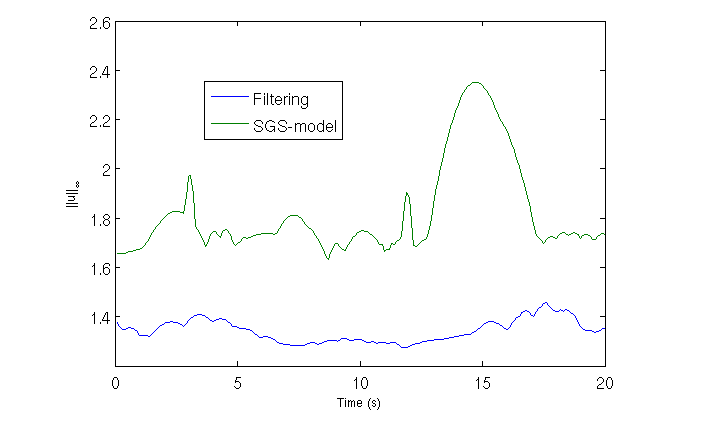
\includegraphics[width=0.6\textwidth]{Figures/maxvel.png}
    \caption{$||\mathbf{u}||_{\infty}$ as a function of time, the green line represents the 
simulation with the dynamic smagorinsky SGS-model and the blue line represents the filtering 
with $\alpha = 0.05$ and a quadratic decay on the last 3 modes.}
	\label{fig:maxvel}
\end{figure}
%
%
%\begin{figure}[h]
	%\centering
	%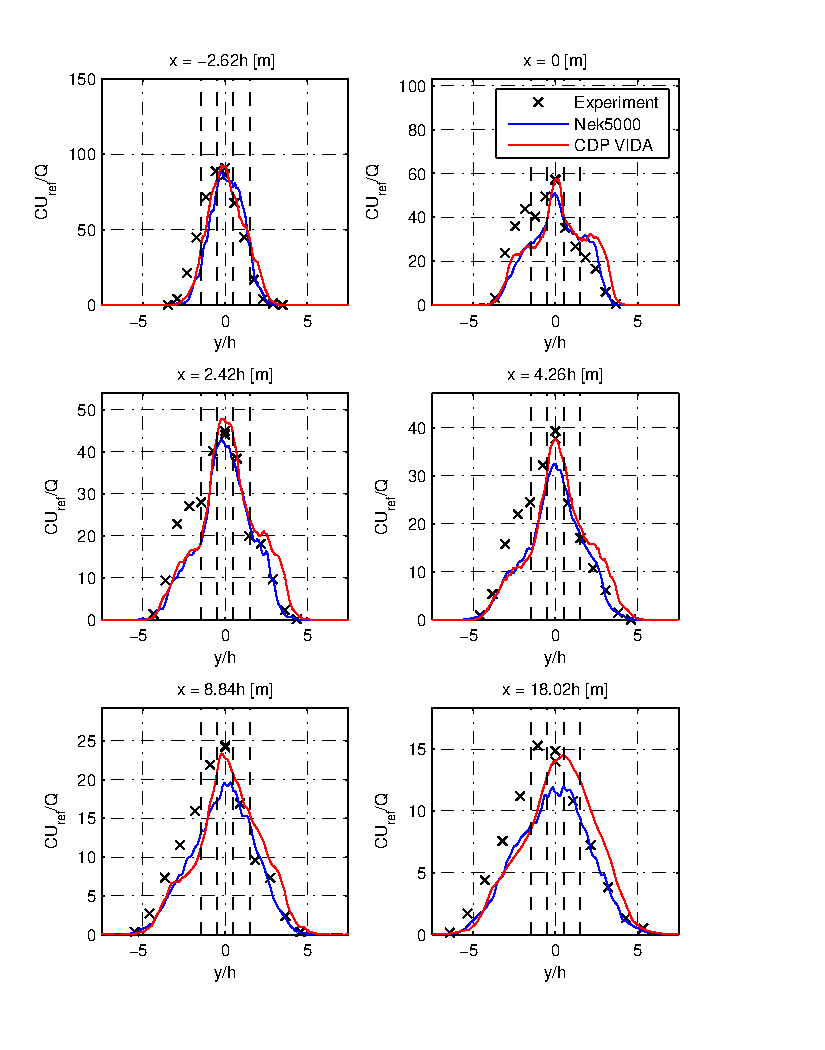
\includegraphics[width=0.8\textwidth]{Figures/NekcH.pdf}
	%\caption{Time-averaged concentration with a sample time of $18.00$ s at $z/H = 0.025$ plotted horizontally and scaled 
	%with the free-stream velocity and emission rate. Compared against wind tunnel data.
%Two dashed lines on either side of the centerline represent the canyon.}
	%\label{fig:cHfilter}
%\end{figure}
%
%
%\begin{figure}[h]
	%\centerline{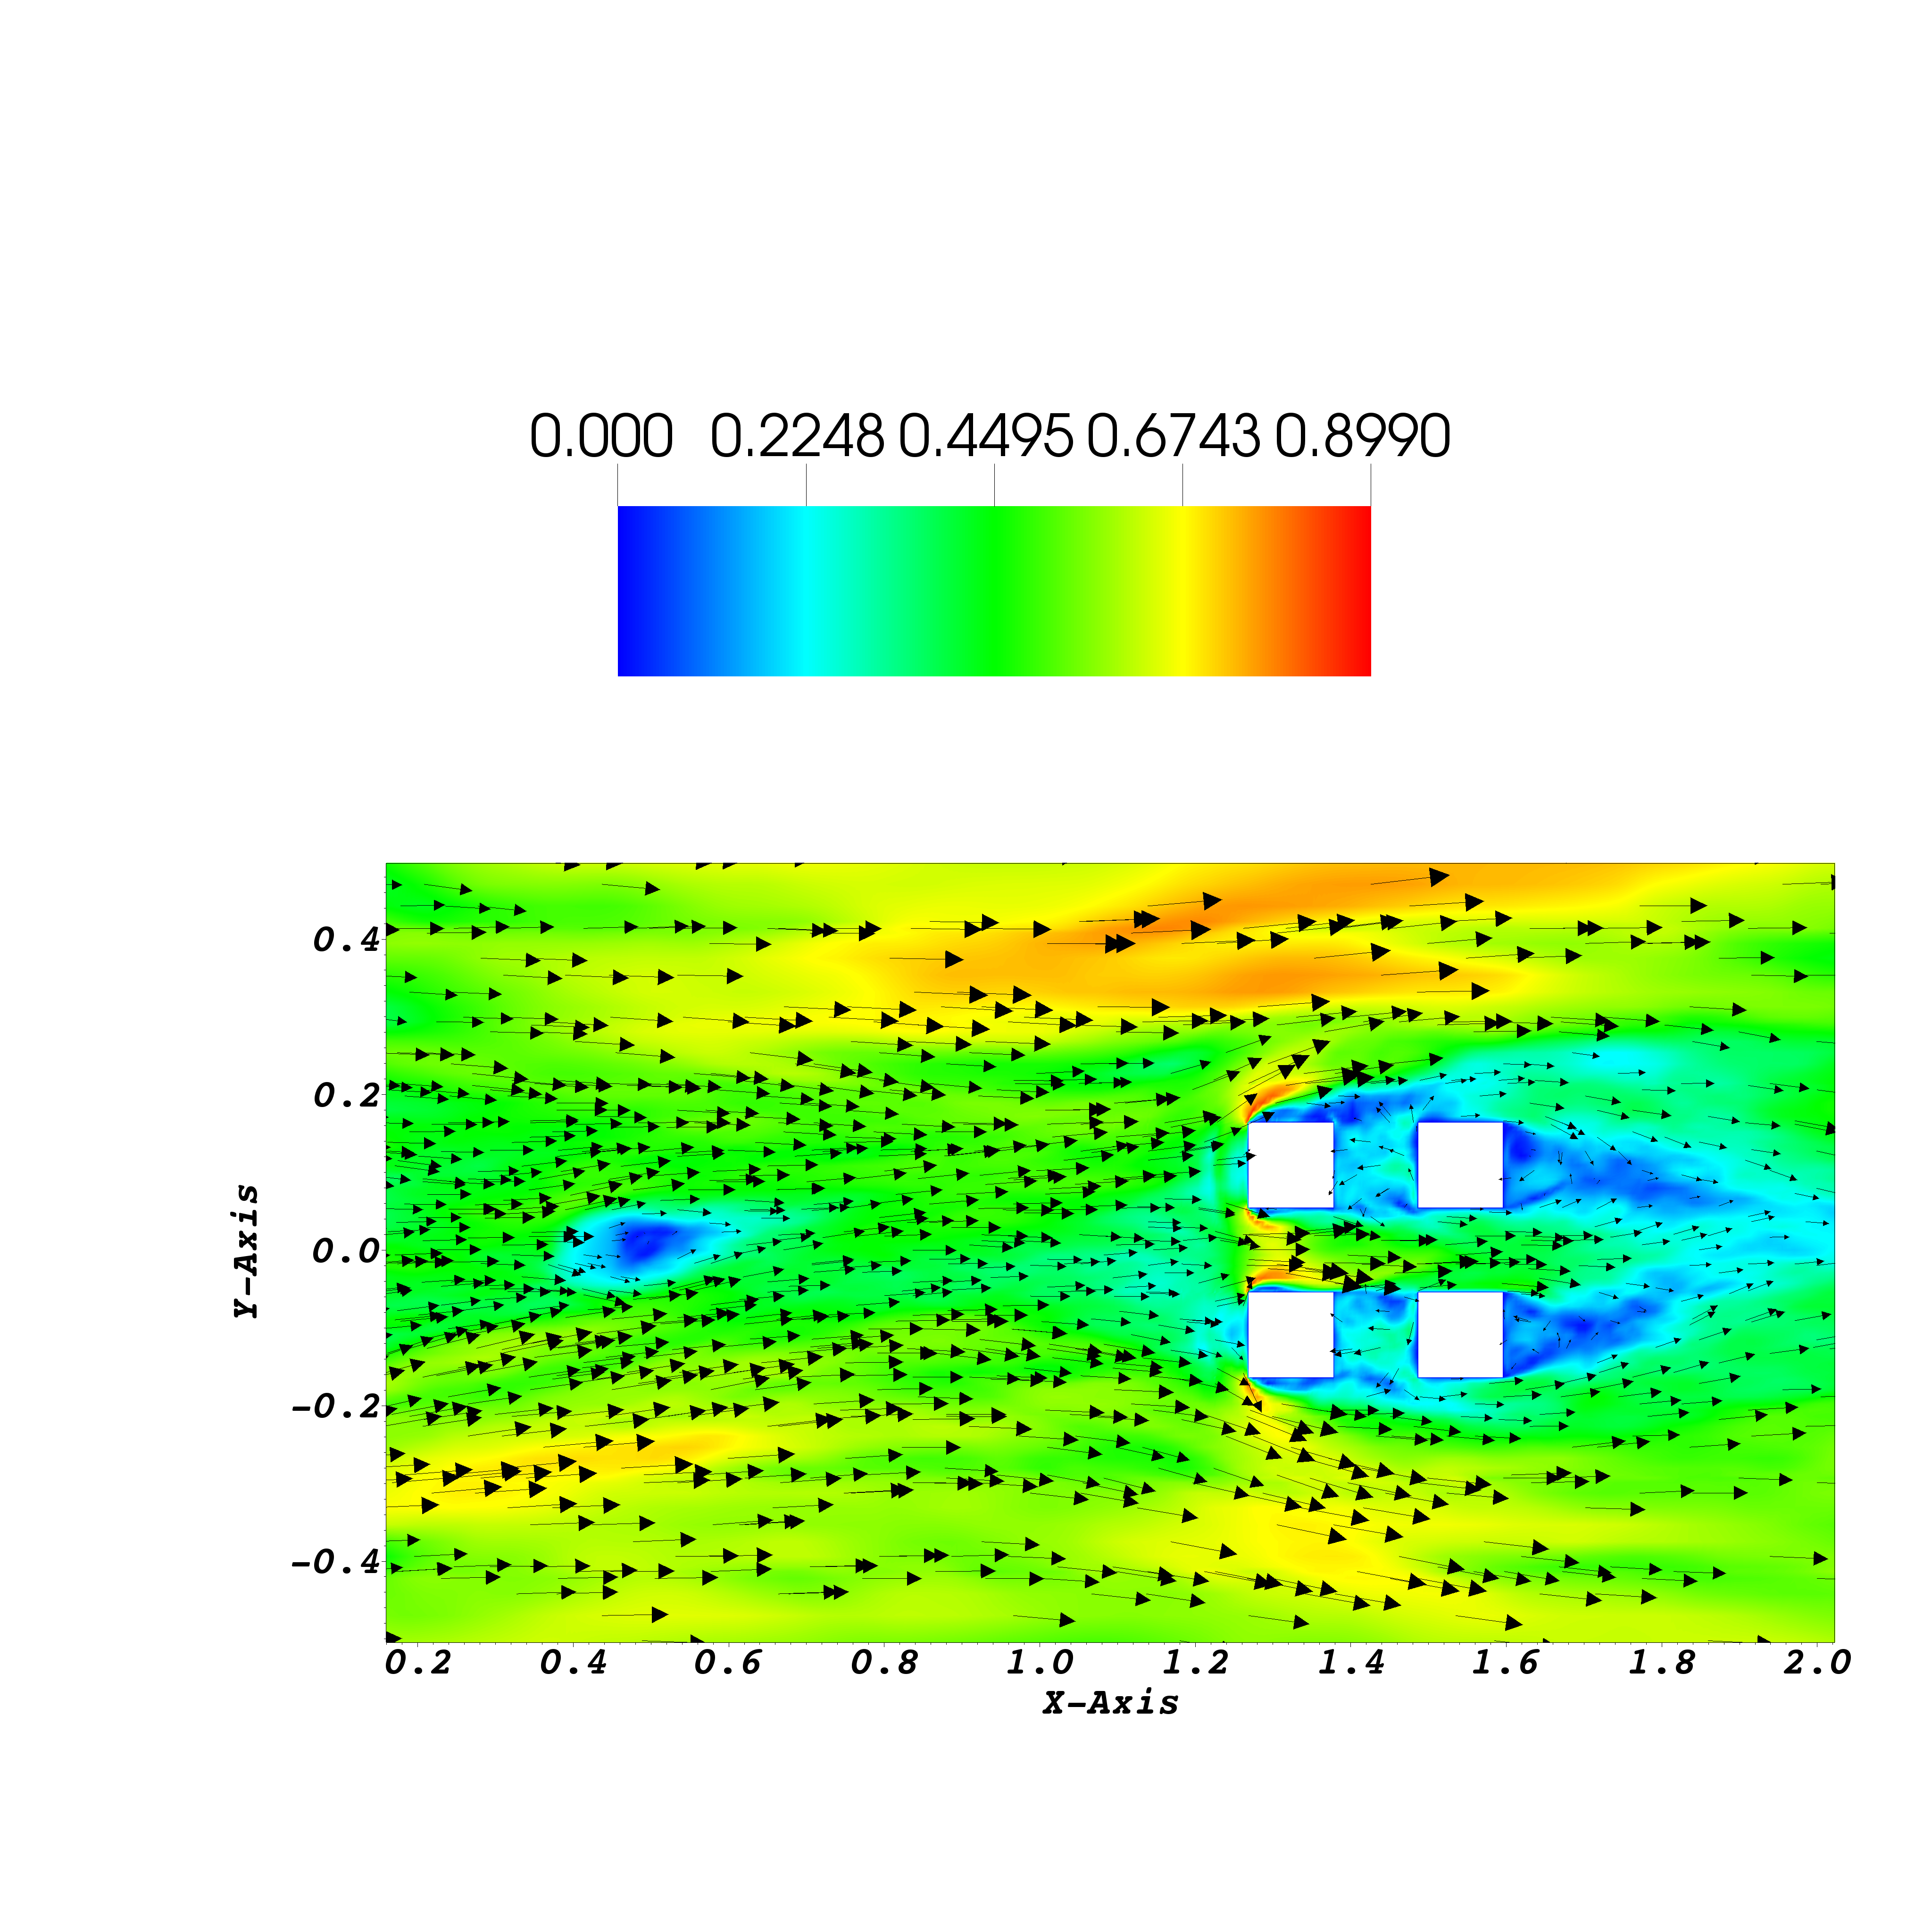
\includegraphics[width=0.8\textwidth]{Figures/vel_field.png}}
	%\caption{velocity field for $z= 0.02$m, around the source and the cubes.}
	%\label{fig:vel_field}
%\end{figure}
%

%\colorbox{green}{redo these simulation in case they were started to early.}
%
%\begin{figure}[h]
	%\centering
	%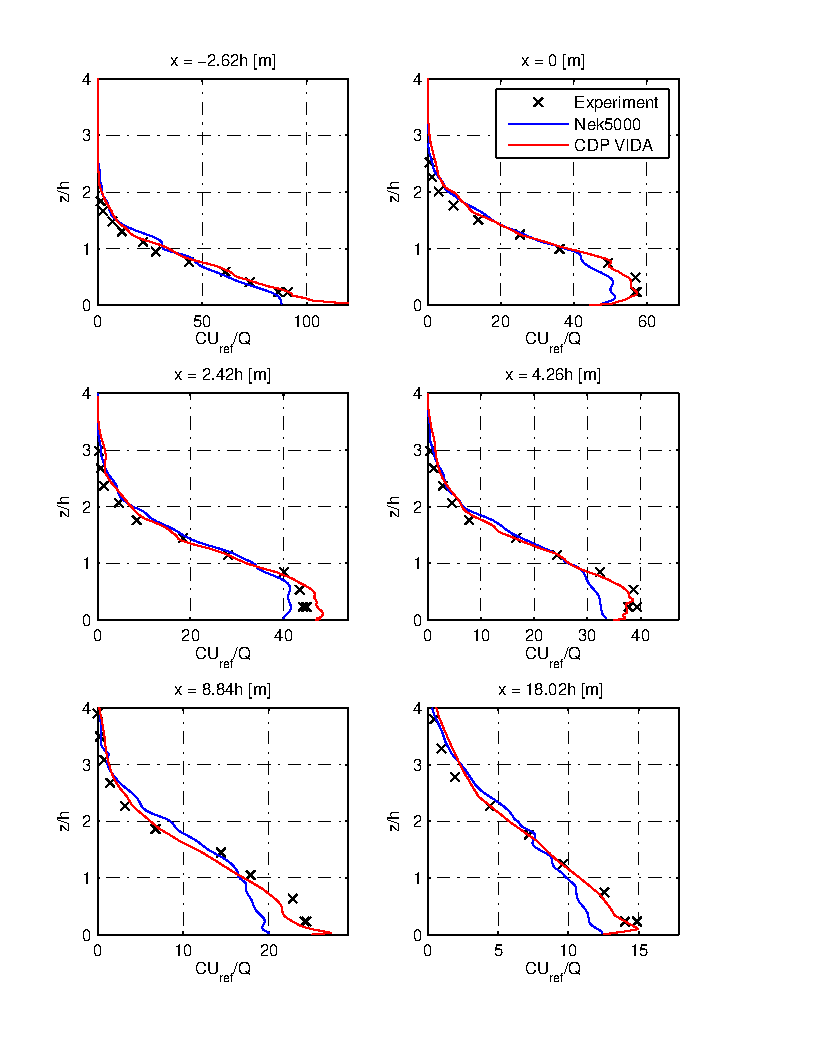
\includegraphics[width=0.8\textwidth]{Figures/NekcV.pdf}
	%\caption{Time-averaged concentration with a sample time of $18.00$ s at $y = 0$ plotted
    %vertically and scaled 
	%with the free-stream velocity and emission rate. Compared against wind tunnel data.
%Two dashed lines on either side of the centerline represent the canyon.}
	%\label{fig:cVfilter}
%\end{figure}
%
%
%\begin{figure}[h]
	%\centering
	%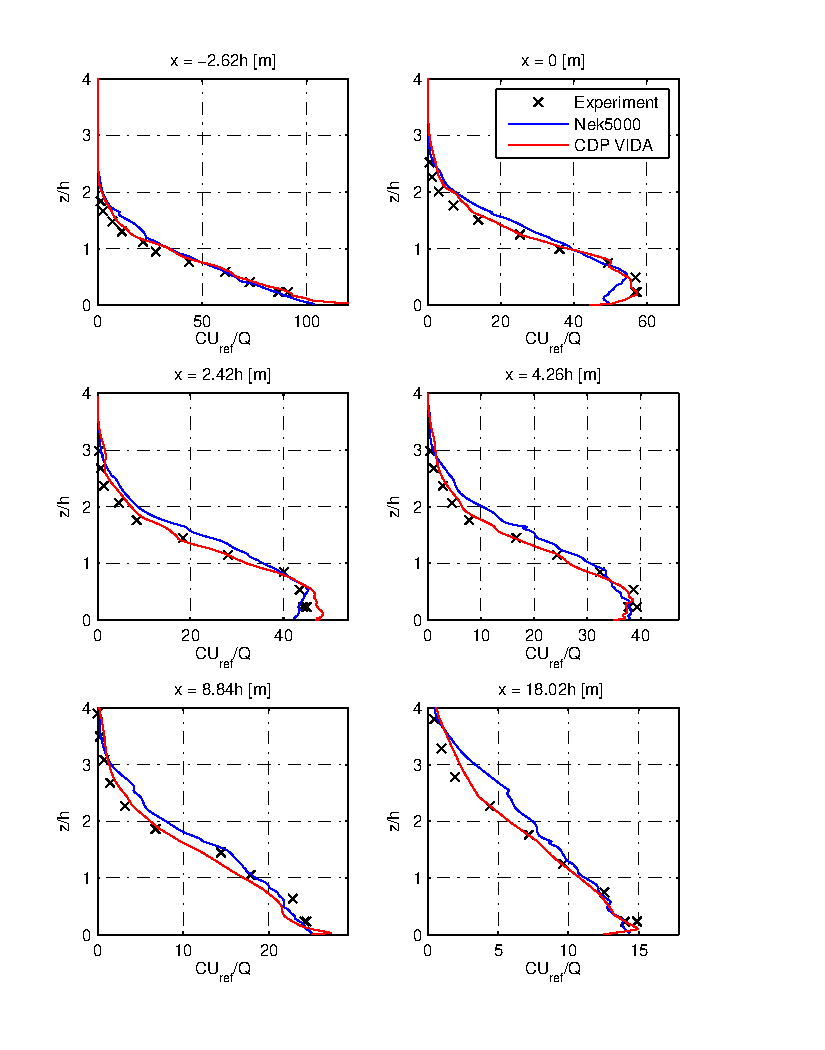
\includegraphics[width=0.8\textwidth]{Figures/Nek_smag_cV.pdf}
	%\caption{Time-averaged concentration with a sample time of $22.00$ s at $y = 0$ plotted
    %vertically and scaled 
	%with the free-stream velocity and emission rate. Compared against wind tunnel data.
%Two dashed lines on either side of the centerline represent the canyon.}
	%\label{fig:cVsmag}
%\end{figure}
%
%
%\begin{figure}[h]
	%\centering
	%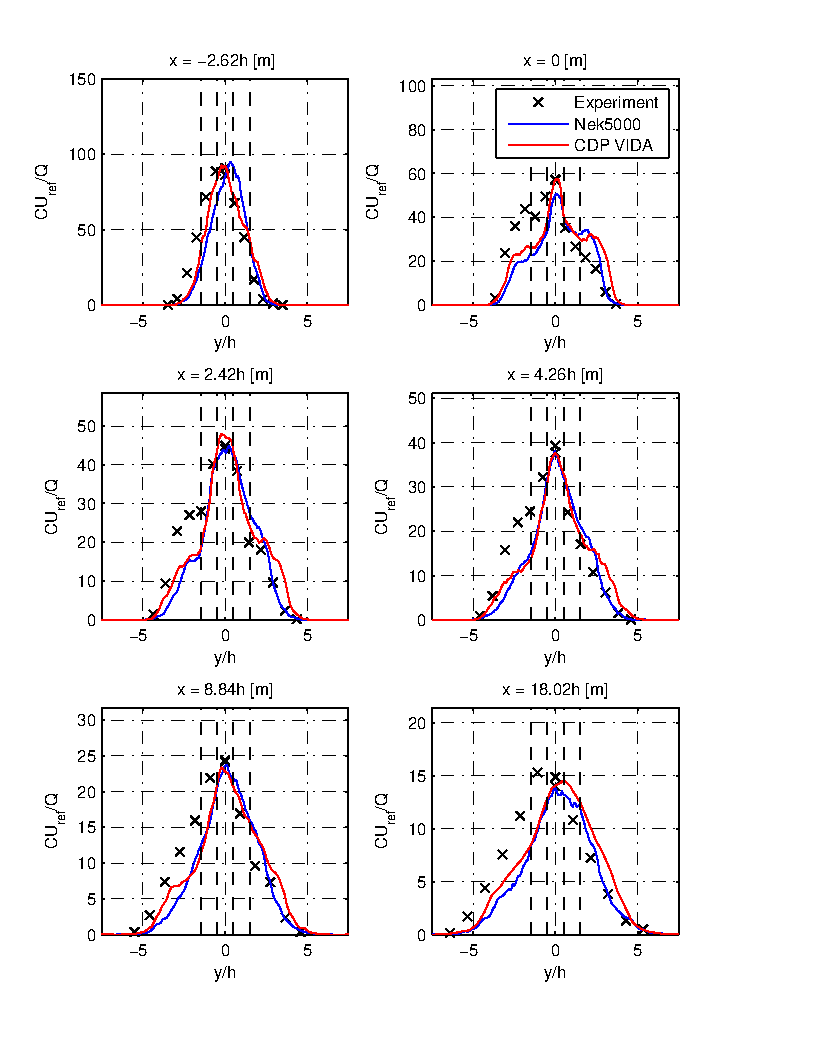
\includegraphics[width=0.8\textwidth]{Figures/Nek_smag_cH.pdf}
	%\caption{Time-averaged concentration with a sample time of $22.00$ s at $y = 0$ plotted
    %vertically and scaled 
	%with the free-stream velocity and emission rate. Compared against wind tunnel data.
%Two dashed lines on either side of the centerline represent the canyon.}
	%\label{fig:cVsmag}
%\end{figure}
%
\newpage
\begin{figure}[h]
    \centering
    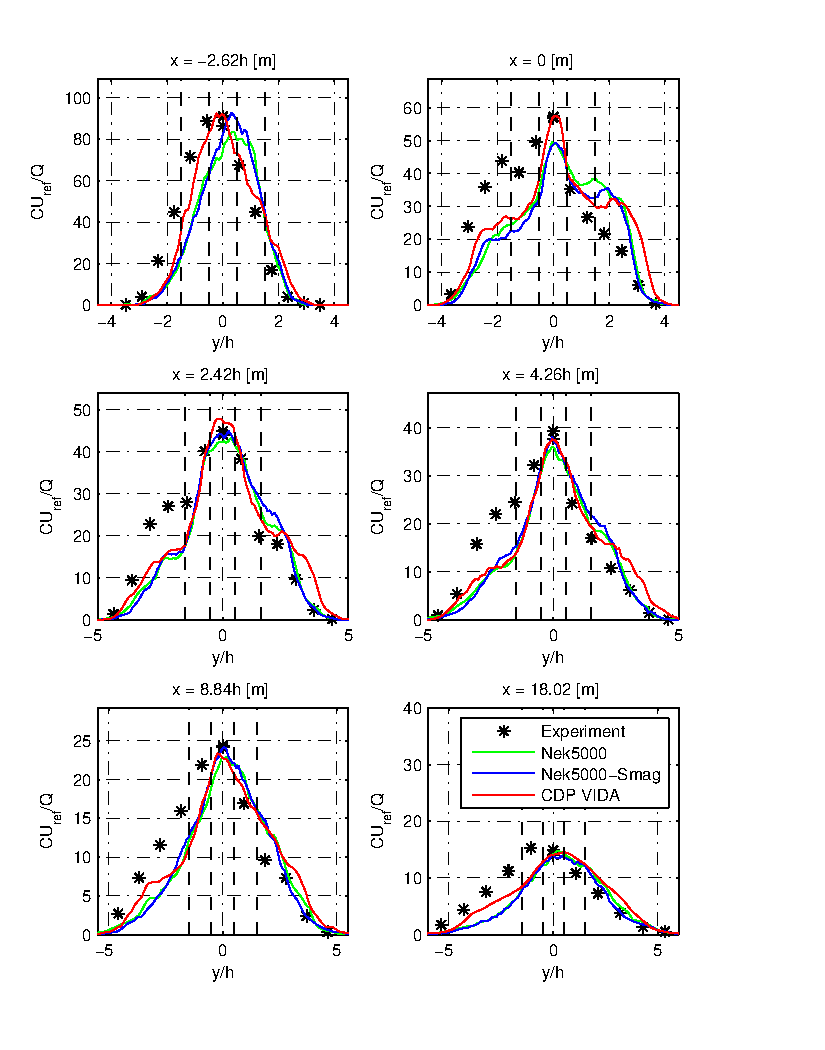
\includegraphics[width=0.8\textwidth]{Figures/NekcH_all.pdf}
    \caption{Time-averaged concentration with a sample time of $22.00$ s at $y = 0$ plotted
    vertically and scaled 
    with the free-stream velocity and emission rate. Compared against wind tunnel data.
Two dashed lines on either side of the centerline represent the canyon.}
    \label{fig:cHall}
\end{figure}

Figure~\ref{fig:cHall} shows the scaled concentration along the dotted lines in~\ref{fig:layout}. 
According to this figure Nek does indeed capture the important features of the mean concentration.
At the two first measurement lines the results are slightly skewed to the right, this is to some degree 
also the case for the CDP simulations but not for the experiment. A possible explanation could be that 
the inflow condition favours one of the sides of the domain, or simply that the sampling time is not 
sufficiently long. 
%Along the second measurement line which is placed in the middle of the 4 cubes Nek5000 
%estimates a concentration peak lower than both the reference solutions.  

The results also indicate that the difference between the SGS-model and filtering are not that large,
if anything the SGS-model shows a tendency to estimate lower concentration peaks. This could be a 
result of too much smoothing due to the turbulent viscosity.

\newpage
\begin{figure}[h]
    \centering
    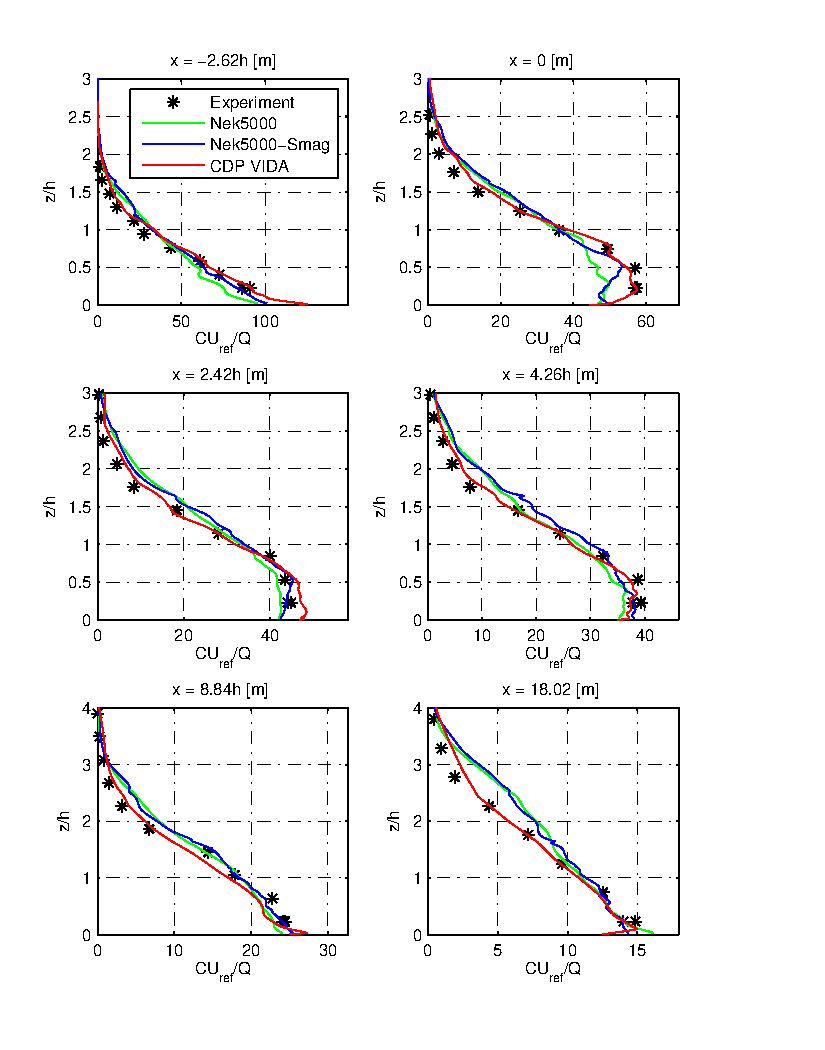
\includegraphics[width=0.8\textwidth]{Figures/NekcV_all.pdf}
    \caption{Time-averaged concentration with a sample time of $22.00$ s at $y = 0$ plotted
    vertically and scaled 
    with the free-stream velocity and emission rate. Compared against wind tunnel data.
Two dashed lines on either side of the centerline represent the canyon.}
    \label{fig:cVall}
\end{figure}
The concentration along the vertical measurement lines is plotted in figure~\ref{fig:cVall} and overall 
Nek5000 provides good results according to the reference solutions. The largest difference is found close 
to the wall right in the middle of the cubes. In particular the simulation including the SGS-model 
underestimates the concentration in this domain. It is known that the Dynamic smagorinsky model does not 
perform that well close to the wall which could be a partial explanation to this. Along with the fact that 
the $P_NP_N$ spitting errors also could be significant close to the wall.


%\begin{figure}[h]
    %\centering
    %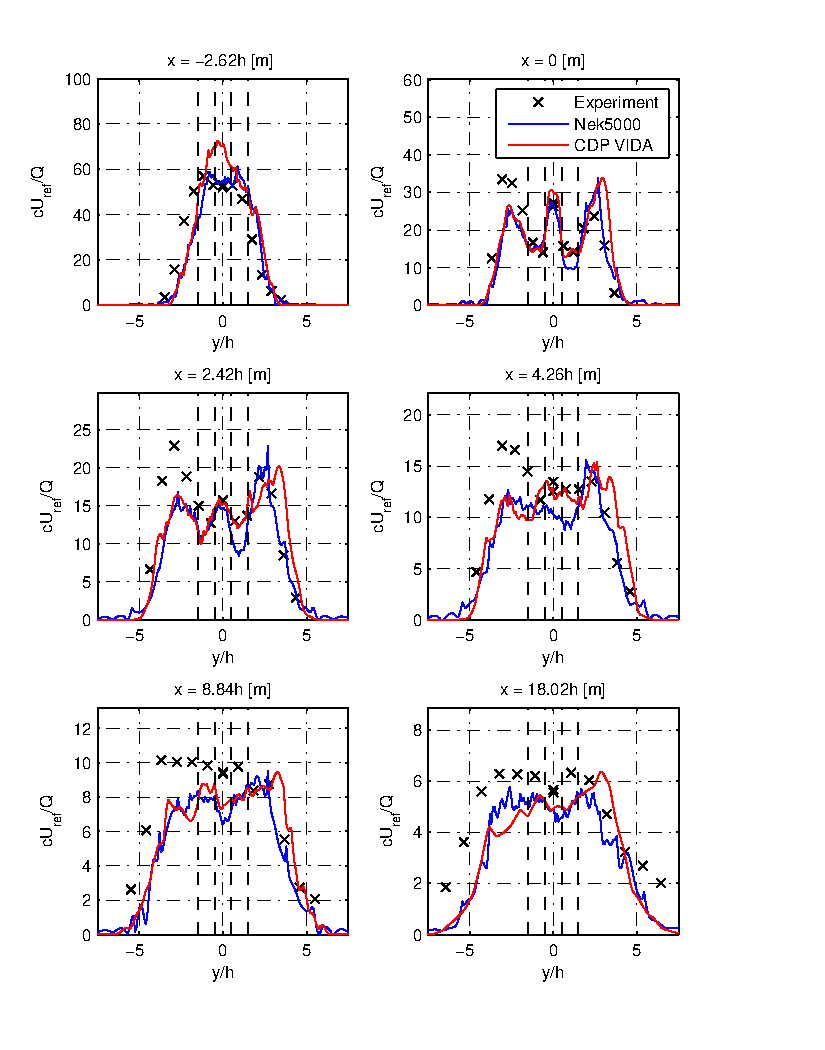
\includegraphics[width=0.8\textwidth]{Figures/Nek_smag_cfluctH.pdf}
    %\caption{Time-averaged concentration with a sample time of $22.00$ s at $y = 0$ plotted
    %vertically and scaled 
    %with the free-stream velocity and emission rate. Compared against wind tunnel data.
%Two dashed lines on either side of the centerline represent the canyon.}
    %\label{fig:cVsmag}
%\end{figure}


\section{Discussion and Conclusion}
\colorbox{green}{How did Nek perform overall, user-friendly ?,correctness,speed etc.}

